\documentclass[a4paper,14pt]{article}


% настройка языка 
\usepackage[utf8]{inputenc}
\usepackage[english, russian]{babel}

% настройка параметров листа
\usepackage[height=297mm, width=210mm, left=3cm, top=2cm, right=1cm, bottom=3cm]{geometry}

% добавление надписей и картинок на фон
\usepackage{eso-pic}

% получение кол-ва листов в файле
\usepackage{lastpage}

% для добавления надписей в рамку
\usepackage[absolute,overlay]{textpos}

% изменение формата номера figure
\usepackage{amsmath}

% настройка подписей к картинкам и таблицам
\usepackage{caption}

% добавляет отступ к 1-ому абзацу после раздела
\usepackage{indentfirst} 

% работа с таблицами
\usepackage{tabularx}

% добавление гиперссылок
\usepackage{hyperref}

% работа с изображениями
\usepackage{graphicx}

% работа с позицией для figure
\usepackage{float}

% добавление предварительных вычислений перед выводом в файл
\usepackage{calc}

% добавление картинок в качестве фона
\usepackage{background}



\captionsetup[figure]{name={Рисунок},labelsep=endash} 
\captionsetup[table]{name={Таблица},labelsep=endash} 

\numberwithin{figure}{section}
\numberwithin{table}{section}

\setlength{\parindent}{12.5mm} 



\newcommand{\chipher}{
        {\fontsize{16pt}{16pt}\selectfont  КП.ИИ-21.210572-40 03-01}
}

\newcommand{\theme}{Прогнозирование цен на жилье с использованием модели случайного леса}

\newcommand{\student}{Худик А.А.}

\newcommand{\teacher}{Головко В.А.}


\begin{document}

        \backgroundsetup{
                scale=3,
                color=black,
                opacity=0.1,
                angle=0,
                position=current page.south,
                vshift=5cm,
                hshift=0cm,
                contents={}
        }
        \setcounter{page}{2}
        \pagestyle{empty}


        \renewcommand{\contentsname}{\centering \MakeUppercase{Содержание}}

        \newcommand{\titlePage}{

    \begin{center}
        МИНИСТЕРСТВО ОБРАЗОВАНИЯ РЕСПУБЛИКИ БЕЛАРУСЬ \\
        УЧРЕЖДЕНИЕ ОБРАЗОВАНИЯ \\
        <<БРЕСТСКИЙ ГОСУДАРСТВЕННЫЙ ТЕХНИЧЕСКИЙ УНИВЕРСИТЕТ>> \\
        ФАКУЛЬТЕТ ЭЛЕКТРОННО-ИНФОРМАЦИОННЫХ СИСТЕМ \\
        Кафедра интеллектуальных информационных технологий \\[4cm]
        
            \MakeUppercase{
                {\bf Пояснительная записка \\}
                к курсовому проекту по дисциплине \\
            }
        
            <<Модели решения задач в интеллектуальных системах>> \\
            Тема: <<\theme>> 
            \\[.5cm]
            
            \chipher \\[4cm]
            
    \end{center}

    \begin{flushright}
        \begin{minipage}{0.35\textwidth}
            \begin{flushleft}
                Листов: \pageref{LastPage} \\[1cm]
                {\bf Выполнил:} \\
                студент 4-го курса, \\
                ФЭИС, \\
                группы ИИ-21 \\
                \student \\
                {\bf Проверил:} \\
                \teacher
            \end{flushleft}
        \end{minipage}
    \end{flushright}

    \vfill 

    \begin{center}
        Брест \the\year
    \end{center}

    \newpage
}



        \newcommand{\contentTablePage}{
    
    % шифр
    \begin{textblock*}{12cm}(8.5cm,25.8cm) 
        \centering 
        \chipher
    \end{textblock*}    

    % лист 3
    \begin{textblock*}{1.5cm}(17cm,27.3cm) 
        \centering 
        3
    \end{textblock*}   

    % листов общее кол-во
    \begin{textblock*}{2cm}(18.5cm,27.3cm) 
        \centering 
        \pageref{LastPage}
    \end{textblock*}  
    
    % уо бргту
    \begin{textblock*}{5cm}(15.5cm,28.3cm) 
        \centering 
        УО <<БрГТУ>>
    \end{textblock*} 

    % тема работы
    \begin{textblock*}{7cm}(8.5cm,26.8cm) 
        \centering 
        \theme
    \end{textblock*} 

    % мое фио
    \begin{textblock*}{2.3cm}(3.74cm,26.85cm) 
        \centering 
        {\fontsize{8pt}{9pt}\selectfont \student}
    \end{textblock*} 

    % фио преподавателя
    \begin{textblock*}{2.3cm}(3.74cm,27.35cm) 
        \centering 
        {\fontsize{9pt}{9pt}\selectfont \teacher}
    \end{textblock*} 


    % вставляем рамку
    % \AddToShipoutPictureBG{

    %     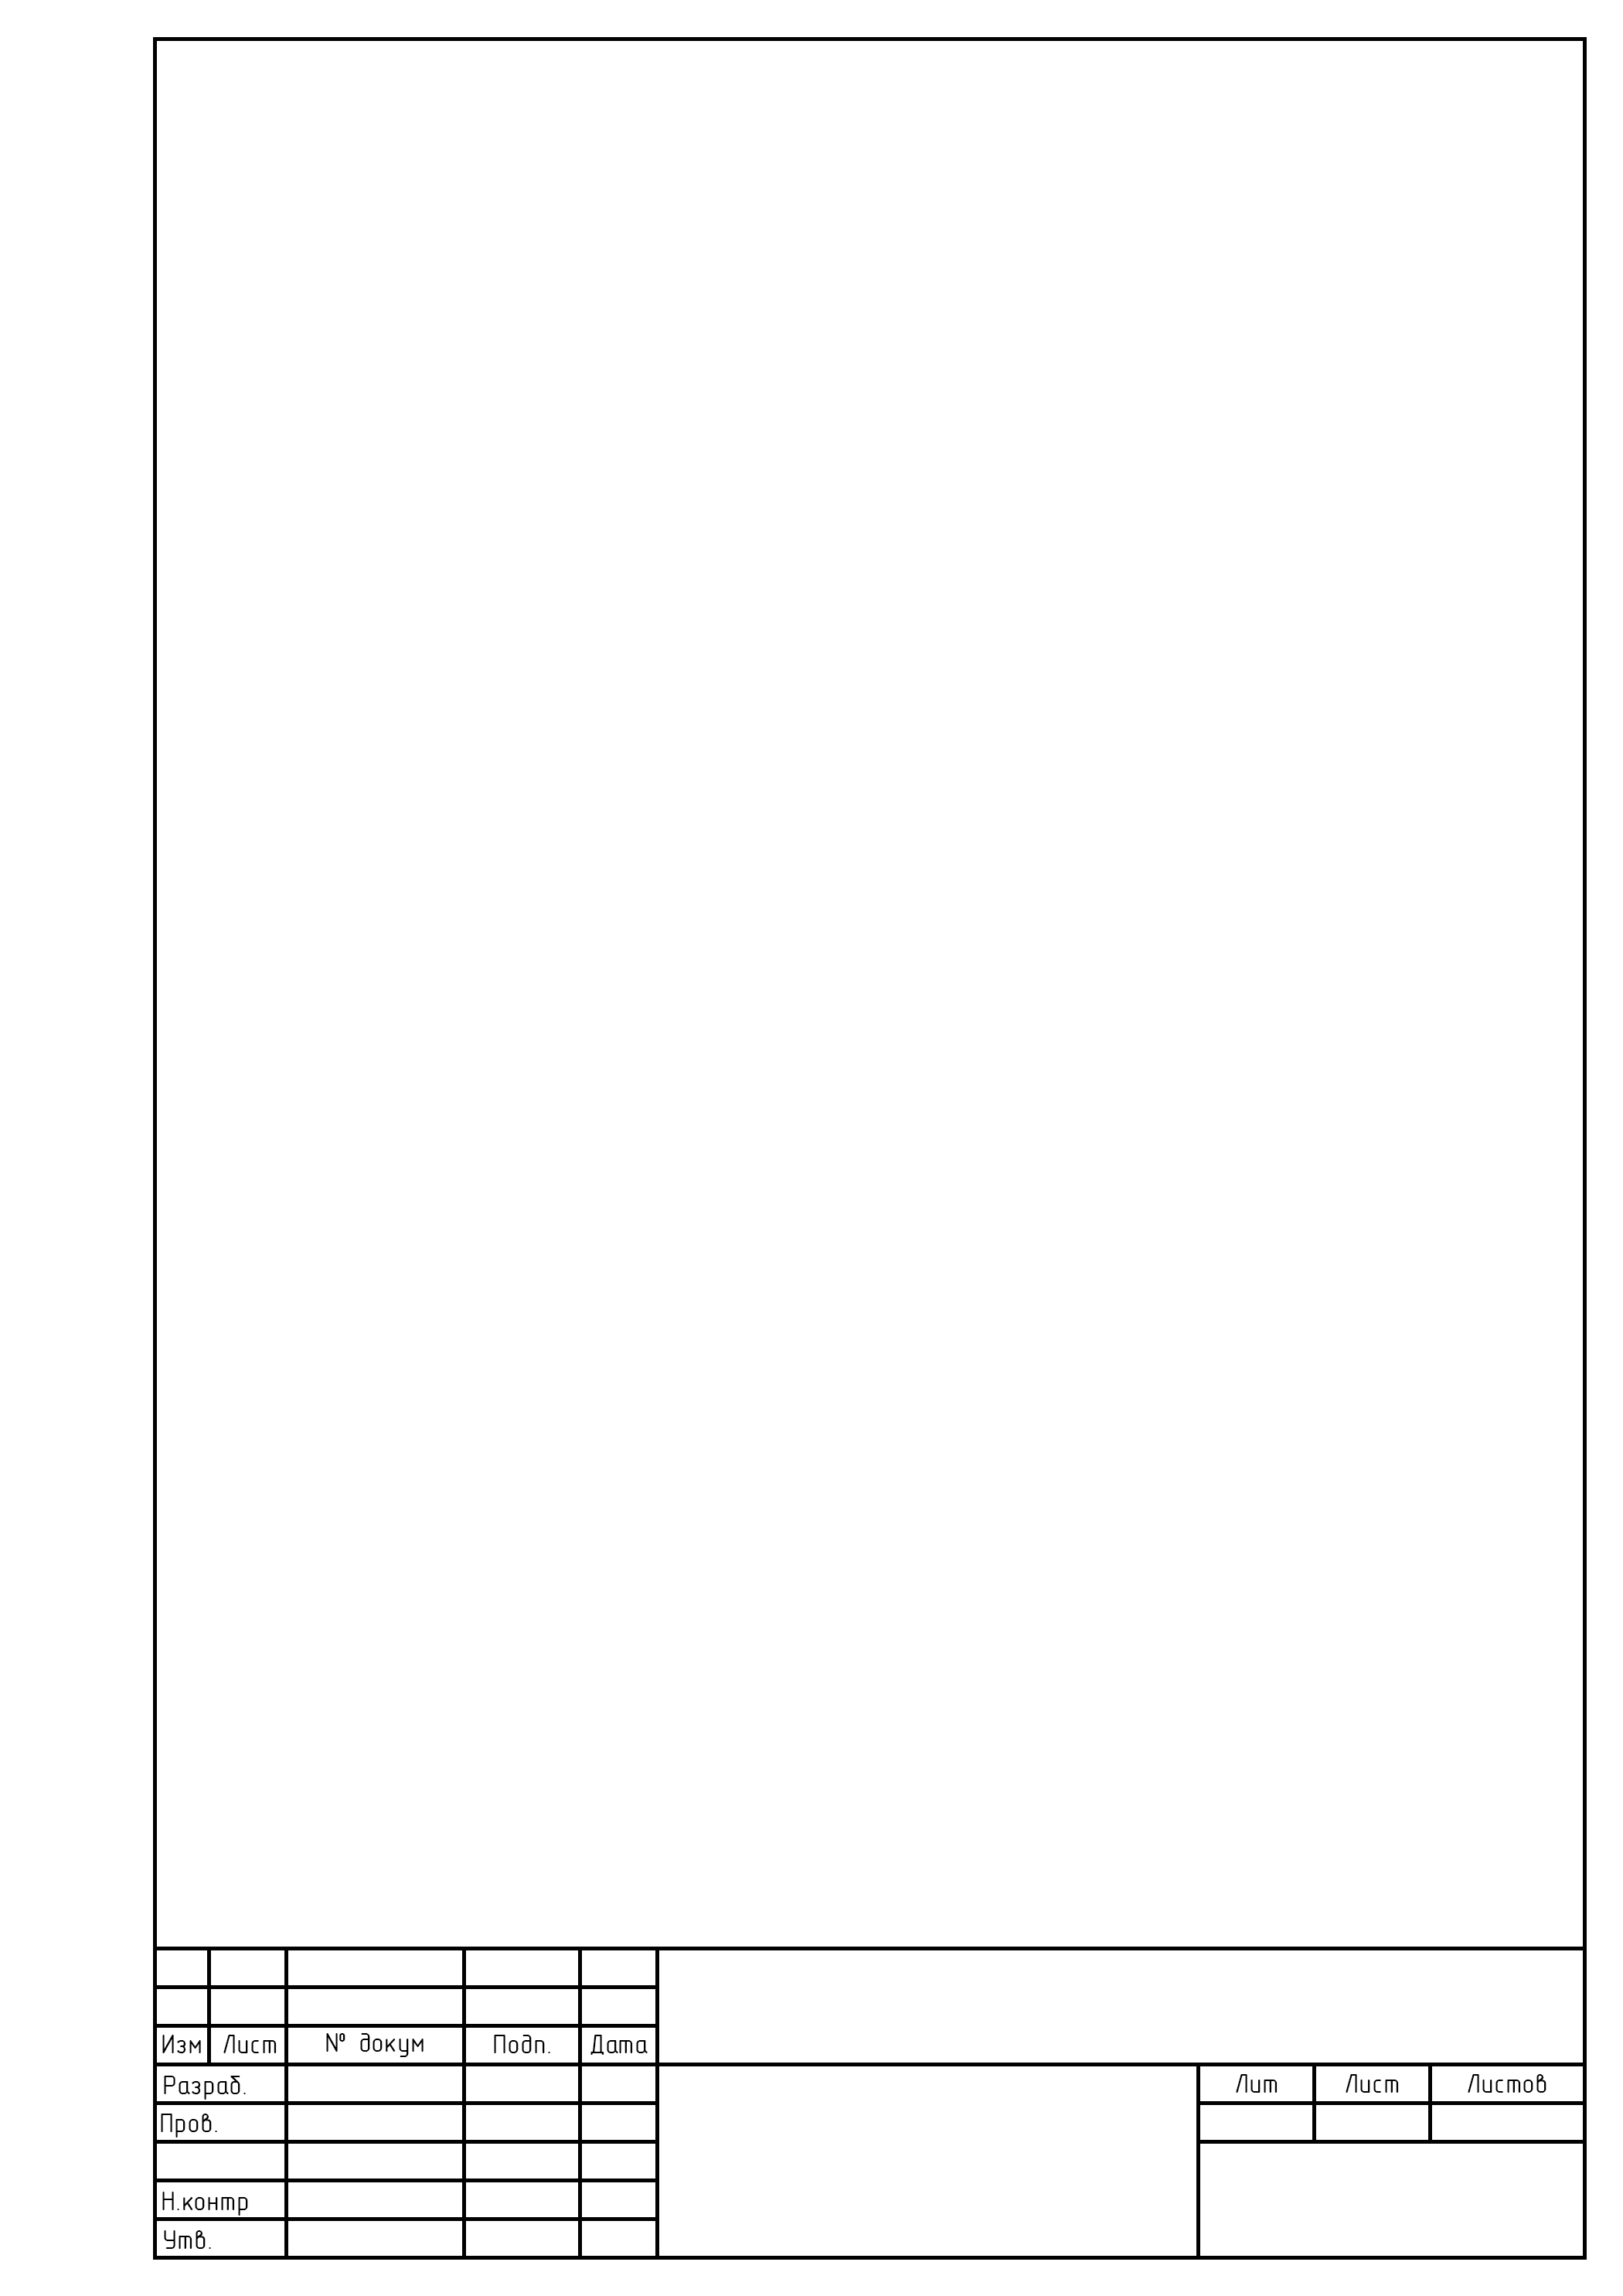
\includegraphics[width=\paperwidth,height=\paperheight]{border/border22.png}
    % }
    \backgroundsetup{
        scale=1,
        color=black,
        opacity=1,
        angle=0,
        position=current page.center,
        vshift=0cm, hshift=0cm,
        contents={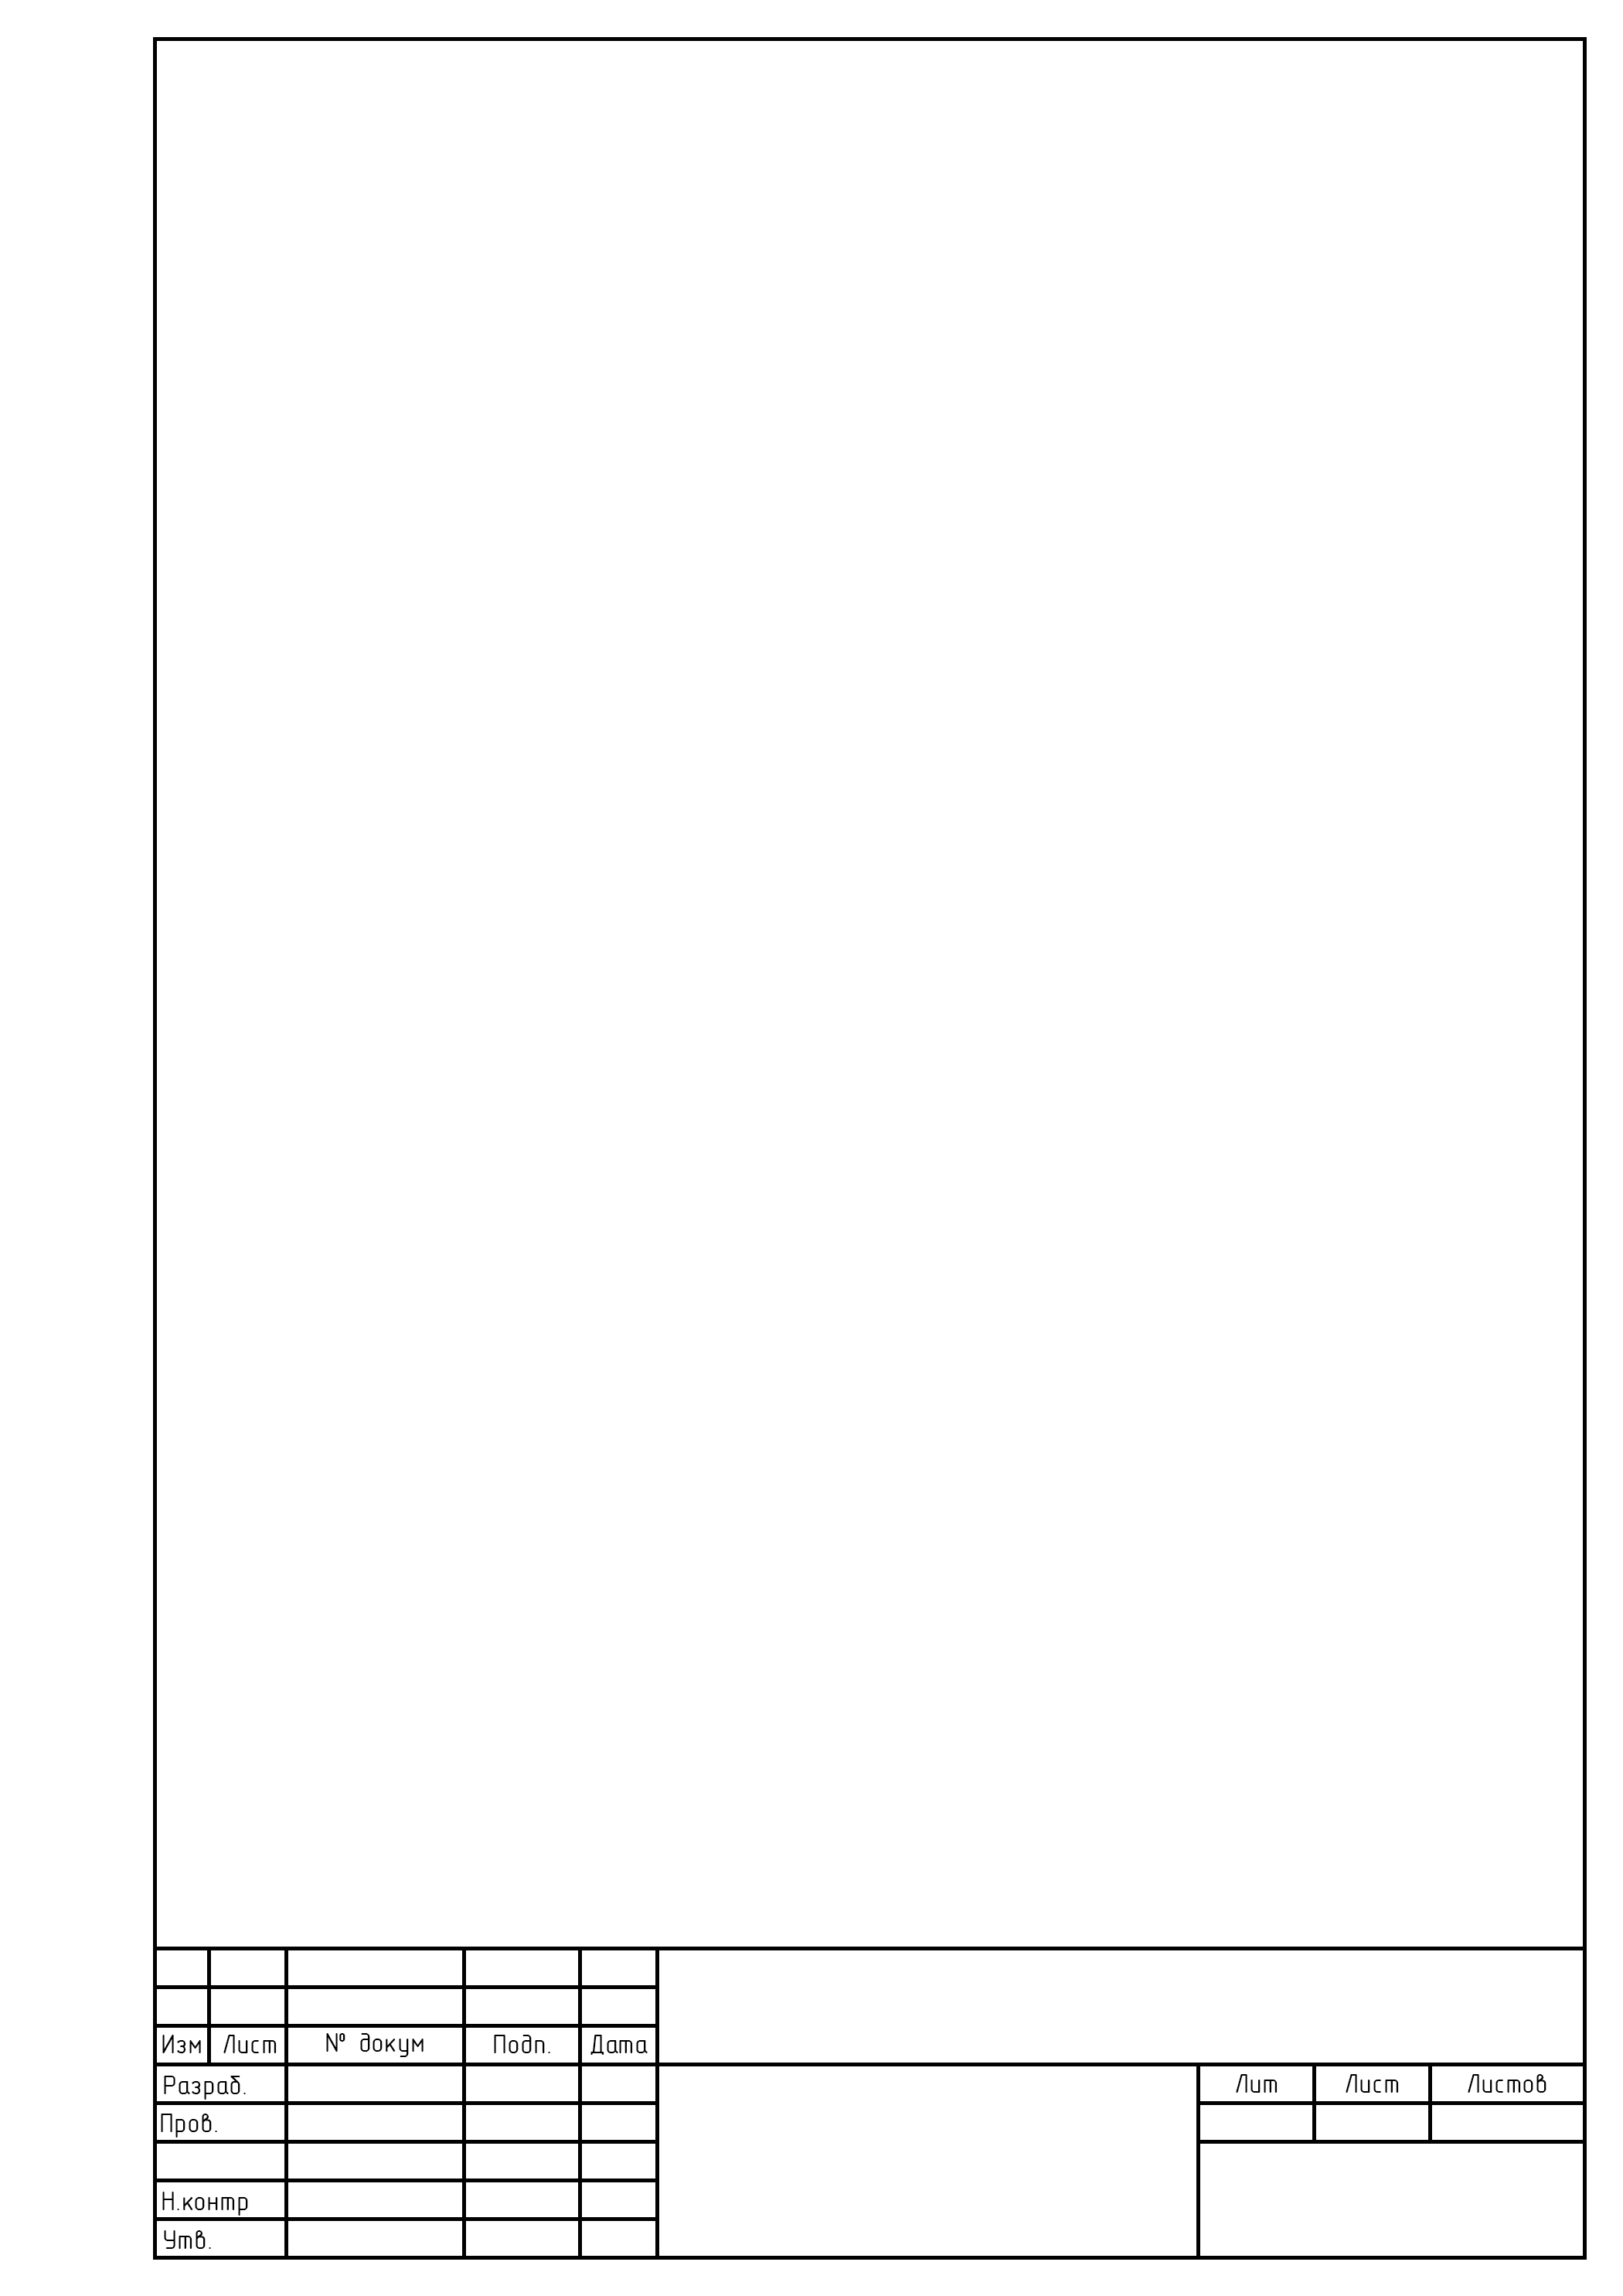
\includegraphics[width=\paperwidth,height=\paperheight]{border/border22.png}}
    }

    % номер для следующей страницы
    \AddToShipoutPicture{
                \begin{textblock*}{1cm}(19.5cm,28.6cm) 
                        \centering 
                        \number\numexpr\thepage+1\relax
                \end{textblock*}
        }
    
    % содержание
    \tableofcontents

    \newpage
    \ClearShipoutPicture

    \backgroundsetup{
                scale=3,
                color=black,
                opacity=0.1,
                angle=0,
                position=current page.south,
                vshift=5cm,
                hshift=0cm,
                contents={}
        }
}
        \newcommand{\content}{
    

    

    % добавляем нумерацию
    \AddToShipoutPicture{
        \begin{textblock*}{1cm}(19.5cm,28.6cm) % Ширина блока, координаты (x, y)
                \centering 
                \number\numexpr\thepage+1\relax
        \end{textblock*}
    }

    % добавляем шифр
    \AddToShipoutPicture{
        \begin{textblock*}{10cm}(9cm,28.2cm) % Ширина блока, координаты (x, y)
            \centering
            \chipher
        \end{textblock*}
    }

    % шифр на 1ый лист
    \begin{textblock*}{10cm}(9cm,28.2cm) % Ширина блока, координаты (x, y)
        \centering
        \chipher
    \end{textblock*}

    \section{\MakeUppercase{Введение}}
    {
        В современном мире стремительного развития технологий обработки и анализа данных задача прогнозирования цен на жилье становится особенно актуальной. Это открывает новые возможности для использования методов машинного обучения, улучшения качества оценки объектов недвижимости и оптимизации процессов ценообразования. Прогнозирование цен играет ключевую роль для покупателей, продавцов, инвесторов и специалистов в сфере недвижимости, предоставляя им точные и обоснованные данные для принятия решений.

Создание моделей прогнозирования цен на жилье, таких как случайный лес, позволяет учитывать множество факторов, включая площадь, расположение, возраст здания и другие важные параметры. Использование библиотек, таких как TensorFlow, дает возможность разрабатывать сложные алгоритмы, способные анализировать большие объемы данных и обеспечивать высокую точность предсказаний. Такие подходы не только повышают уровень автоматизации процессов, но и способствуют более эффективному управлению недвижимостью.

Кроме того, внедрение моделей машинного обучения в анализ цен на жилье создает новые перспективы для развития интеллектуальных систем. Например, улучшение точности прогноза цен способствует созданию платформ, которые помогают пользователям оценивать рыночную стоимость объектов в реальном времени. Это делает рынок недвижимости более прозрачным и доступным для всех участников.

Применение моделей случайного леса в TensorFlow для прогнозирования цен на жилье является важным шагом к расширению использования искусственного интеллекта в повседневной жизни. Такие технологии позволяют значительно улучшить процесс принятия решений и способствуют созданию инновационных решений в области анализа и обработки данных.
    }
    \newpage

\newpage
\section{\MakeUppercase{Постановка задачи}}

Целью данной работы является разработка системы прогнозирования цен на жилье, основанной на методах машинного обучения. В качестве базовой модели будет использоваться алгоритм случайного леса, реализованный с помощью библиотеки TensorFlow, который будет обучаться на специализированном датасете, содержащем данные о недвижимости, включая такие параметры, как площадь, расположение, возраст здания и другие характеристики.

Задачи, которые необходимо решить в рамках проекта:
\begin{enumerate}
    \item \textbf{подготовка набора данных:} \\
    Необходимо собрать и подготовить набор данных, содержащий параметры объектов недвижимости и их рыночную стоимость. Данные должны быть очищены от нерелевантной или некорректной информации. Важно учесть разнообразие характеристик, влияющих на стоимость, а также сбалансированность набора данных. Также требуется подготовить данные для последующей подачи в модель, включая нормализацию и обработку пропущенных значений. 
    \item \textbf{выбор архитектуры модели:} \\
    Проанализировать существующие реализации алгоритмов случайного леса и выбрать подходящую конфигурацию для решения задачи. Это включает в себя настройку таких параметров, как количество деревьев, глубина деревьев и критерии разбиения.
    \item \textbf{обучение модели:} \\
    Обучить модель случайного леса на подготовленных данных, используя TensorFlow. Это позволит построить модель, способную учитывать нелинейные зависимости между характеристиками объектов и их ценой.
    \item \textbf{оценка качества работы модели:} \\
    После обучения модели необходимо провести её тестирование на независимом наборе данных, используя метрики, такие как MSE (Mean Squared Error) и RMSE (Root Mean Squared Error). Анализ результатов поможет определить точность и надежность прогноза, а также выявить возможные направления для улучшения модели.
\end{enumerate}

\newpage
\section{\MakeUppercase{Выбор и описание используемых инструментов}}
{

Для решения задачи прогнозирования цен на жилье с использованием случайного леса в TensorFlow были выбраны следующие инструменты и библиотеки: 
    \begin{itemize}
        \item \textbf{TensorFlow:} основной фреймворк для разработки и обучения моделей машинного обучения. TensorFlow обеспечивает эффективное выполнение вычислений и предоставляет множество инструментов для создания сложных моделей, включая реализацию алгоритма случайного леса;
        \item \textbf{Seaborn:} библиотека для визуализации данных. Применялась для анализа и визуализации взаимосвязей между характеристиками недвижимости, что помогло выявить ключевые факторы, влияющие на стоимость жилья;
        \item \textbf{Pandas:} библиотека для работы с табличными данными. Использовалась для загрузки и предобработки набора данных, включая очистку, нормализацию и преобразование данных в формат, подходящий для обучения модели;
        \item \textbf{Matplotlib:} библиотека для построения графиков. Использовалась для визуализации распределений данных и анализа результатов предсказаний модели;
    \end{itemize}
    Эти библиотеки обеспечили эффективный процесс работы над проектом, включая предобработку данных, обучение модели случайного леса и визуализацию результатов. Такой набор инструментов является оптимальным для решения задачи прогнозирования цен на жилье.
}

\newpage
\section{\MakeUppercase{Обучение нейронной сети}}
В данном разделе описаны этапы обучения модели для прогнозирования цен на жилье с использованием случайного леса в TensorFlow, а также процесс подготовки данных.
{
\subsection{Подготовка данных}
Подготовка данных — один из ключевых этапов в процессе обучения модели. Для эффективного прогнозирования цен на жилье, на основе исходных данных о недвижимости, были выполнены следующие шаги:
\begin{itemize}
    \item \textbf{скачивание данных:} для работы был использован набор данных, содержащий информацию о недвижимости, включая такие параметры, как площадь, количество комнат, возраст здания, расположение, наличие парковки и другие характеристики. Данные были загружены в формате CSV с помощью библиотеки Pandas. Пример данных:
    \newline \newline \includegraphics[scale=0.5]{ {/Users/andrewhudik/Downloads/Screenshot 2024-12-29 at 9.39.02 PM.png} }
    \item \textbf{очистка данных:} на этапе предварительной обработки были устранены пропущенные значения, некорректные или выбросные данные. Например, строки с некорректными значениями (отрицательная площадь или цена) были удалены, а пропуски заменены на медианные значения по соответствующему признаку;   
    \item \textbf{анализ данных:} с использованием библиотек Seaborn и Matplotlib был проведен анализ данных, чтобы определить взаимосвязи между характеристиками объектов и их ценой. Построены диаграммы корреляции, распределения и ящичные диаграммы для выявления ключевых факторов;    
    \item \textbf{разделение на тренировочную и тестовую выборки:} данные были разделены на тренировочную и тестовую выборки. Это разделение обеспечило независимость тестовых данных, необходимых для оценки качества модели;    
\end{itemize}
}

\subsection{Выбор архитектуры нейронной сети}

Для задачи прогнозирования цен на жилье была выбрана модель случайного леса, реализованная с использованием \textit{TensorFlow Decision Forests}. Этот выбор был обусловлен следующими преимуществами:
\begin{itemize}
    \item \textbf{Обработка табличных данных:} случайный лес является одним из наиболее подходящих алгоритмов для работы с табличными данными, содержащими числовые и категориальные признаки.
    \item \textbf{Интерпретируемость:} благодаря структуре модели можно легко анализировать вклад каждого признака в итоговое предсказание, что особенно важно в задачах прогнозирования цен.
    \item \textbf{Устойчивость к переобучению:} модель случайного леса хорошо справляется с задачами, где признаки могут быть скоррелированы или содержать выбросы.
\end{itemize}

\subsection*{Характеристики модели}
\begin{itemize}
    \item \textbf{Архитектура дерева:} модель состоит из нескольких деревьев решений, объединенных в ансамбль. Каждое дерево строится на случайной подвыборке данных, а разбиения узлов деревьев основаны на случайно выбранных подмножествах признаков. Это позволяет снизить вероятность переобучения и повысить обобщающую способность.
    \item \textbf{Глубина деревьев:} максимальная глубина деревьев была ограничена, чтобы избежать переобучения, но при этом позволить модели улавливать сложные зависимости в данных.
    \item \textbf{Количество деревьев:} было выбрано оптимальное количество деревьев, обеспечивающее баланс между временем обучения и точностью предсказаний.
\end{itemize}

\subsection*{Функция активации и методы обучения}
Хотя модель случайного леса не использует нейронные сети, структура обучения аналогична некоторым аспектам глубокого обучения:
\begin{itemize}
    \item \textbf{Активация:} для преобразования признаков и их влияния на конечное предсказание модель использует нелинейные разбиения в узлах деревьев, аналогичные нелинейностям в нейронных сетях.
    \item \textbf{Оптимизация гиперпараметров:} для достижения максимальной точности была проведена оптимизация гиперпараметров модели (глубина деревьев, количество деревьев, размер подвыборки данных).
\end{itemize}

Использование случайного леса в сочетании с \textit{TensorFlow Decision Forests} позволяет интегрировать классический подход с преимуществами современного фреймворка машинного обучения, что обеспечивает высокую производительность модели при прогнозировании цен на жилье.


\subsection{Обучение нейронной сети}

\begin{enumerate}
    \item \textbf{Создание случайных подвыборок (bootstrap)}  
    Для каждого дерева в ансамбле формируется случайная подвыборка данных из обучающей выборки с возвращением. Это означает, что одни и те же данные могут попасть в подвыборку несколько раз, а некоторые данные могут вовсе не быть выбраны.  
    Такой подход снижает корреляцию между деревьями, так как каждое дерево видит немного разные данные.  

    \item \textbf{Выбор случайного набора признаков}  
    На каждом этапе разбиения дерева выбирается случайное подмножество признаков для поиска оптимального условия разделения. Параметр \texttt{max\_features} управляет размером этого набора:  

    \item \textbf{Построение дерева}  
    Дерево обучается на своей подвыборке, постепенно разделяя данные на узлах:  
    \begin{enumerate}
        \item \textbf{выбор условия разделения:} для каждой вершины рассматриваются все доступные признаки из случайного подмножества. Для каждого признака находятся пороговые значения, минимизирующие ошибку (например, MSE).  
        \item \textbf{разделение:} данные разделяются на две группы (левую и правую ветви) в соответствии с выбранным условием. Этот процесс повторяется до достижения заданной глубины дерева (\texttt{max\_depth}) или пока в листьях не останется минимальное число объектов (\texttt{min\_samples\_leaf}).  
    \end{enumerate}

    \item \textbf{Формирование прогнозов на листьях}  
    Когда дерево достигает листа, оно фиксирует прогноз для объектов, попавших в этот лист. Прогнозом может быть среднее значение целевой переменной для объектов в листе.  

    \item \textbf{Повторение процесса для всех деревьев}  
    Каждый этап (создание подвыборки, выбор признаков, построение дерева) повторяется для каждого дерева в ансамбле. В результате получается множество независимых деревьев, обученных на различных подмножествах данных.  

    \item \textbf{Комбинирование прогнозов}  
    После обучения каждого дерева их прогнозы сохраняются для дальнейшего усреднения. Такой подход снижает вероятность переобучения, поскольку каждое дерево вносит свой уникальный вклад в итоговый результат.  
\end{enumerate}
\newpage
\section{\MakeUppercase{Тестирование нейронной сети}}
В данном разделе рассматриваются этапы тестирования обученной модели для предсказания цен на недвижимость с использованием алгоритма Random Forest. Основной целью тестирования является оценка корректности работы модели, её точности и эффективности. Тестирование включало следующие этапы:

\begin{itemize}
    \item \textbf{Функциональное тестирование}: проверка работы модели на тестовых данных для анализа её способности правильно предсказывать цену недвижимости. Модель должна демонстрировать способность точно и стабильно работать на различных примерах данных, не участвующих в процессе обучения.
    \item \textbf{Оценка качества модели}: после обучения модель тестируется на отложенной выборке. Оценка качества производится с использованием нескольких метрик, которые позволяют получить полное представление о её эффективности. К основным метрикам можно отнести:
    \begin{itemize} 
        \item \textbf{MSE (Mean Squared Error)} — среднеквадратичная ошибка, которая измеряет среднее квадратичное отклонение предсказанных значений от истинных. Это основная метрика для задач регрессии, показывающая, насколько хорошо модель предсказывает целевые значения.
        \item \textbf{R² (коэффициент детерминации)} — метрика, которая показывает, какую часть вариации зависимой переменной объясняет модель. Чем выше значение R², тем лучше модель предсказывает данные.
    \end{itemize}
    Также строится график изменений ошибки на обучающих и валидационных данных по мере увеличения числа деревьев в модели, что позволяет оценить динамику улучшения точности.
    \item \textbf{Тестирование производительности}: проверка времени выполнения модели на тестовом наборе данных, а также анализ её эффективности при обработке больших объёмов данных. Оценка производительности важна для понимания, насколько быстро модель может генерировать предсказания на реальных данных в условиях реального времени.
\end{itemize}

В результате тестирования модель показала хорошую общую точность, особенно при предсказании цен для более распространённых типов недвижимости. Основные ошибки были связаны с домами, которые имели нетипичные характеристики или сильно отличались от представленных в обучающих данных. Для повышения точности в таких случаях планируется дополнительно расширить и улучшить данные, а также провести настройку гиперпараметров модели.
\newpage
\section{\MakeUppercase{Заключение}}
В ходе выполнения курсового проекта была достигнута основная цель — разработана система предсказания цен на жилье с использованием алгоритмов деревьев решений, в частности, модели случайного леса (Random Forest) на базе TensorFlow Decision Forests. Основное внимание было уделено подготовке специализированного датасета, обучению модели и оценке её точности на основе различных метрик.

В процессе работы была реализована модель, которая эффективно предсказывает цену на жилье, используя различные характеристики, такие как площадь, количество комнат, состояние недвижимости и другие. Обучение проводилось на подготовленных данных с использованием метрик средней квадратичной ошибки (MSE), что позволило всесторонне оценить её эффективность. Проведённая настройка гиперпараметров и архитектуры модели позволила достичь высокой точности предсказания.

Использованные методы и технологии продемонстрировали потенциал деревьев решений для решения задач регрессии в области предсказания цен. Разработанная система может быть применена для оценки рыночной стоимости недвижимости, автоматизации процессов анализа рынка жилья и оптимизации принятия решений в сфере недвижимости.

Результаты работы показывают перспективность применения алгоритмов деревьев решений в задачах предсказания и регрессии. Данный проект открывает новые возможности для улучшения точности прогноза в области недвижимости, а также для внедрения таких технологий в реальный бизнес.
\newpage
\section{Список использованной литературы}
\sloppy
{
    \begin{enumerate}
        \item H. W. Tan, W. P. et al. \textit{TensorFlow Decision Forests: A Library for Decision Forests with TensorFlow} [Электронный ресурс]. – Режим доступа: \url{https://www.tensorflow.org/decision_forests}. – Дата доступа: 19.11.2024.
        \item Guo, Y., et al. \textit{The Basics of Decision Trees in Machine Learning} [Электронный ресурс]. – Режим доступа: \url{https://towardsdatascience.com/the-basics-of-decision-trees-in-machine-learning-38c3e2080f9d}. – Дата доступа: 19.11.2024.
        \item Kaggle. \textit{Housing Prices: Advanced Regression Techniques} [Электронный ресурс]. – Режим доступа: \url{https://www.kaggle.com/c/house-prices-advanced-regression-techniques}. – Дата доступа: 19.11.2024.
        \item W. G. Gilks. \textit{Decision Trees for Regression and Classification} [Электронный ресурс]. – Режим доступа: \url{https://machinelearningmastery.com/decision-trees-for-regression-and-classification/}. – Дата доступа: 17.11.2024.
        \item TensorFlow. \textit{TensorFlow Documentation} [Электронный ресурс]. – Режим доступа: \url{https://www.tensorflow.org/docs}. – Дата доступа: 19.11.2024.

    \end{enumerate}
}
}


        \fontsize{14}{17.5}\selectfont    
        
        \titlePage

        \contentTablePage

        % Устанавливаем картинку на фон
    \backgroundsetup{
        scale=1,
        color=black,
        opacity=1,
        angle=0,
        position=current page.center,
        vshift=0cm, hshift=0cm,
        contents={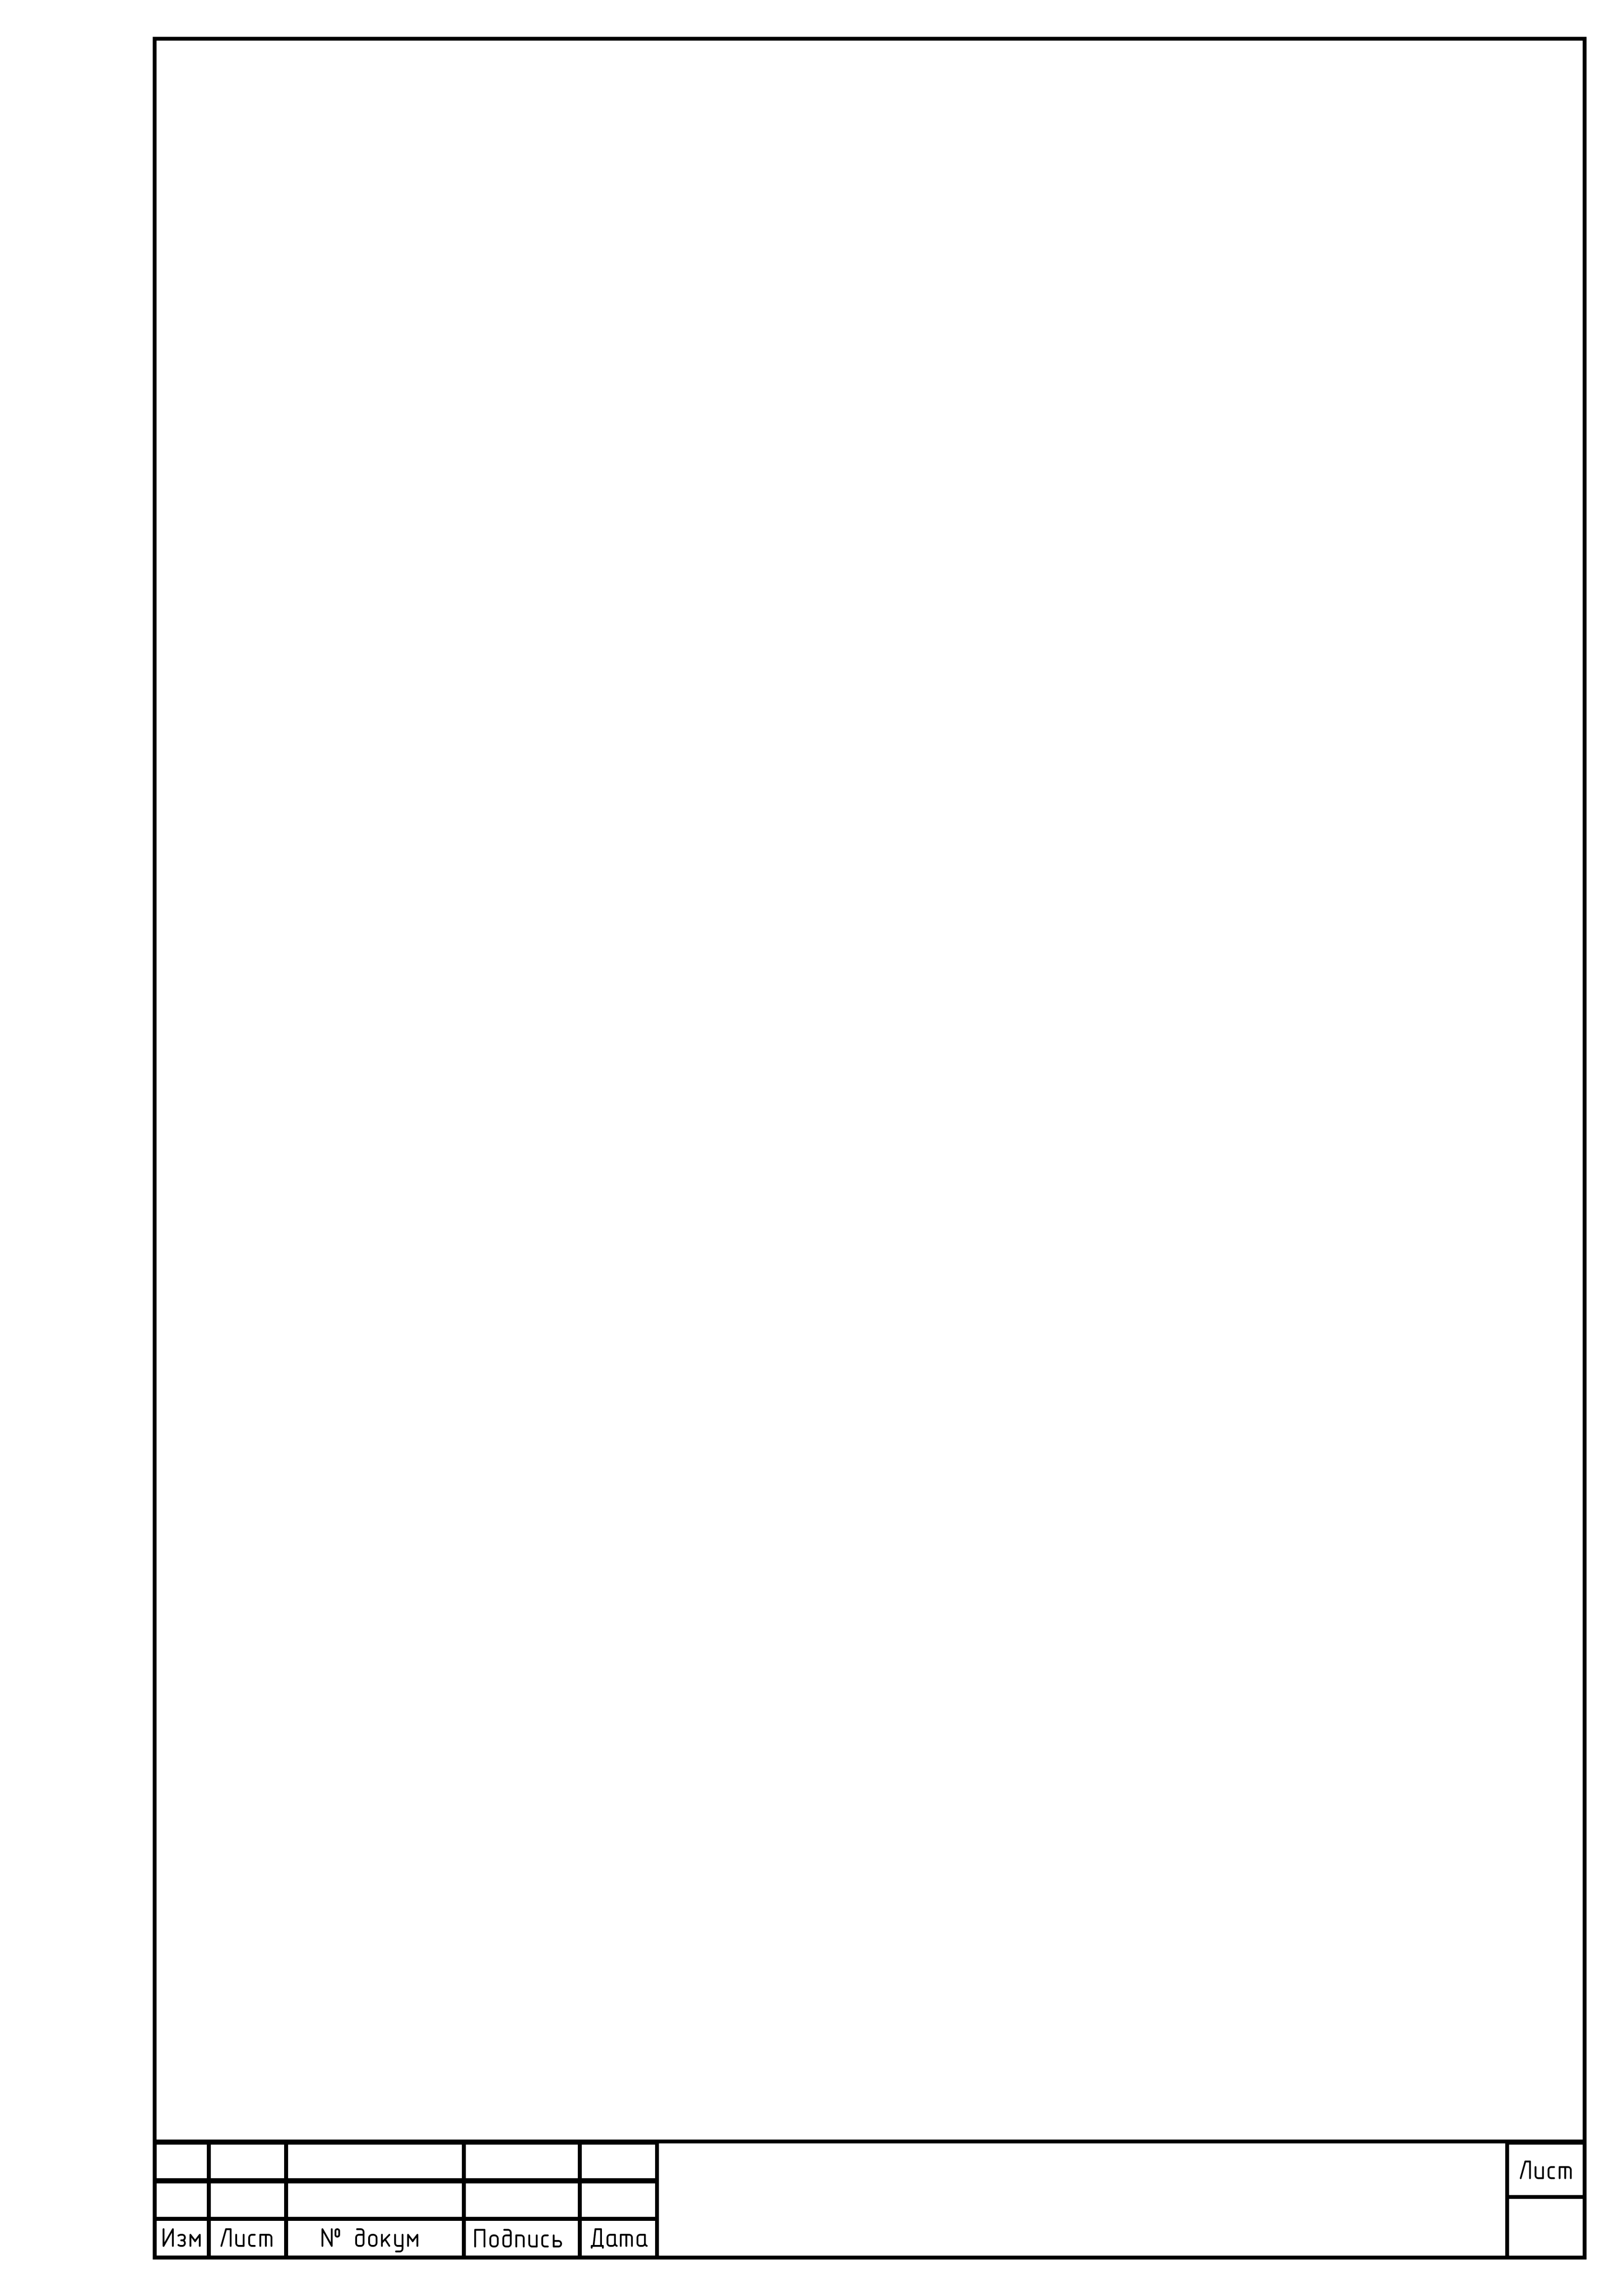
\includegraphics[width=\paperwidth,height=\paperheight]{border/border11.png}}
    }
        \content
    
\end{document}
